% Figure snippets for main.tex. Embed inline, do not \input.

% Figure 1: Schematic of structured regression analogy.
\begin{figure}[htbp]
\centering
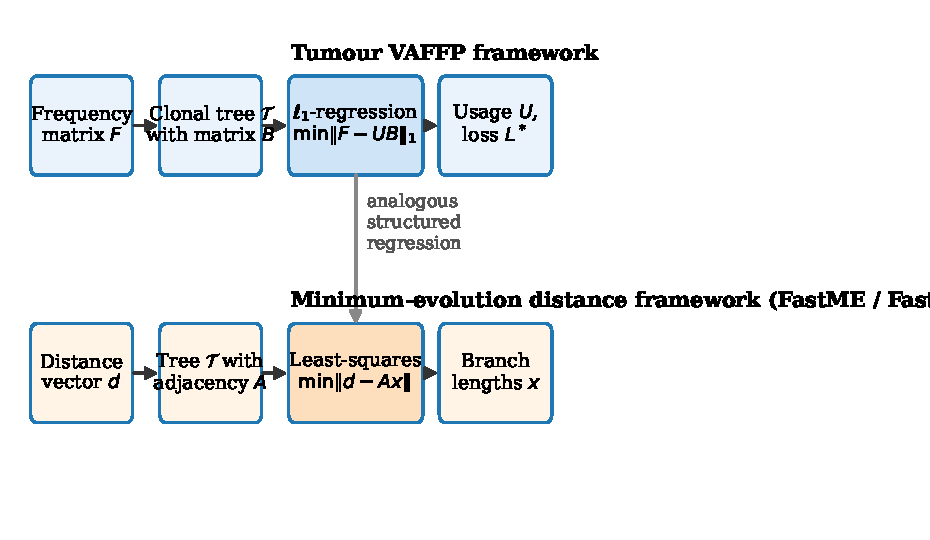
\includegraphics[width=0.9\textwidth]{figures/fig_schematic.pdf}
\caption{Analogous structured-regression problems for a fixed tree topology $\mathcal{T}$. (Top) The $\ell_1$-VAFFP framework for tumour evolution, where the usage matrix $U$ describes the fraction of each clone in every bulk sample and the clonal matrix $B_{\mathcal{T}}$ encodes the genotype of each clone in $\mathcal{T}$. (Bottom) The minimum-evolution framework for distance-based phylogenetics, where the adjacency-like matrix $A_{\mathcal{T}}$ relates the branch-length vector $x$ to the observed distance vector $d$. fastBE transfers the regression-plus-local-search design from distance-based phylogenetics to bulk-tumour phylogenetics.}
\label{fig:schematic}
\end{figure}

% Figure 2: LP speedups.
\begin{figure}[htbp]
\centering
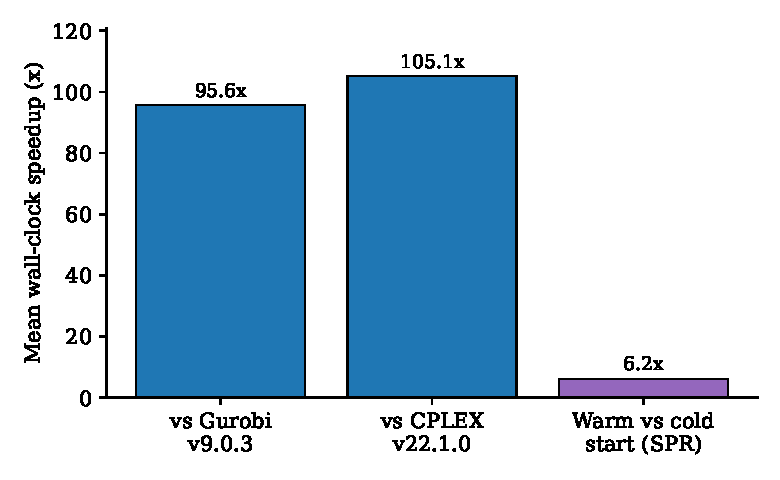
\includegraphics[width=0.7\textwidth]{figures/fig_lp_speedup.pdf}
\caption{Mean wall-clock speedup of our structured $\ell_1$-regression algorithm relative to commercial linear programming solvers across 264 simulated $(F,B)$ instances (Gurobi~v9.0.3: 95.6$\times$; CPLEX~v22.1.0: 105.1$\times$), and mean speedup of warm-start recomputation versus cold-start re-solution after a single random SPR move across 25{,}000 perturbations per instance (6.2$\times$).}
\label{fig:lp_speedup}
\end{figure}

% Figure 3: F1 vs clones.
\begin{figure}[htbp]
\centering
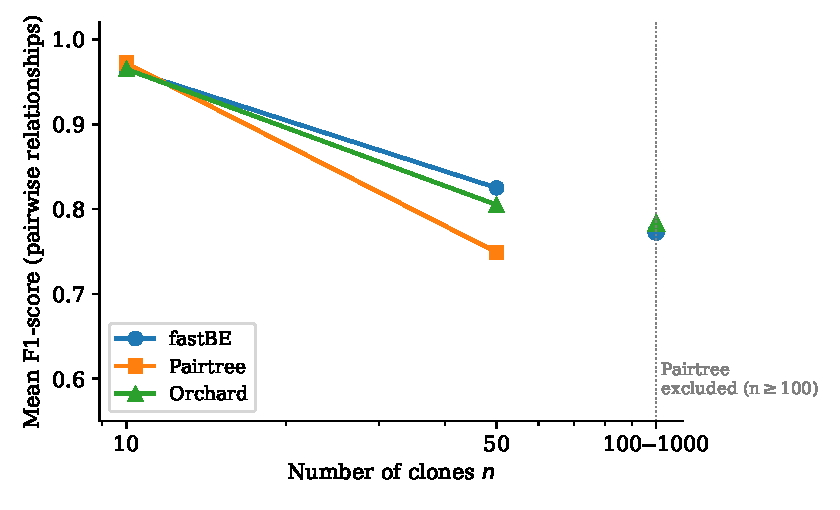
\includegraphics[width=0.75\textwidth]{figures/fig_f1_vs_clones.pdf}
\caption{Mean F1-score of reconstructed pairwise ancestral relationships on simulated data for fastBE, Pairtree and Orchard across regimes. Values at $n=10$ and $n=50$ are exact means over the simulated instances in each regime; the right-most points summarise the large-clone regime $n\in\{100,250,500,1000\}$, where only fastBE and Orchard terminated within the 24-hour time budget. CALDER and CITUP did not scale beyond $n\geq 20$ and are omitted.}
\label{fig:f1_vs_clones}
\end{figure}

% Figure 4: Runtime comparison.
\begin{figure}[htbp]
\centering
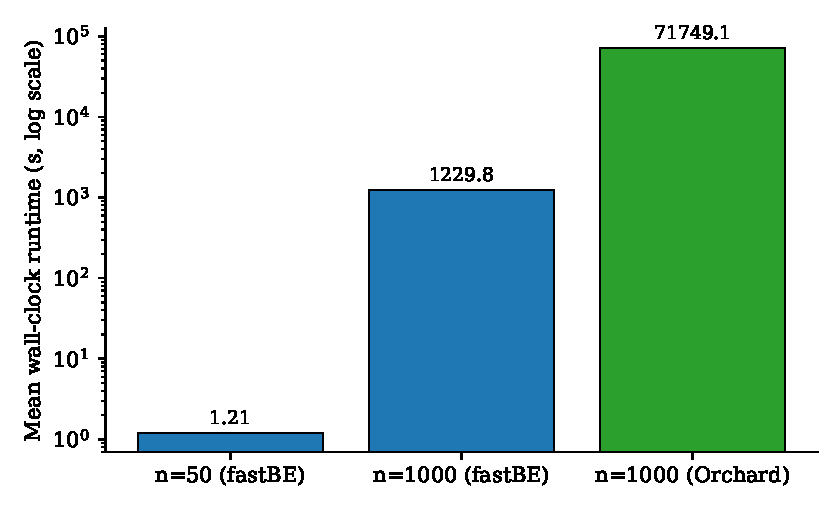
\includegraphics[width=0.7\textwidth]{figures/fig_runtime.pdf}
\caption{Mean wall-clock runtime on simulated instances (logarithmic scale). fastBE completes $n=50$-clone instances in an average of 1.21~s, and $n=1000$-clone instances in 1229.8~s with 24/24 terminations; Orchard required a mean of 71{,}749.1~s and terminated on 19/24 of the same $n=1000$ instances even when allotted 48 hours and a dedicated 32-core processor.}
\label{fig:runtime}
\end{figure}

% Figure 5: Sum-condition violation.
\begin{figure}[htbp]
\centering
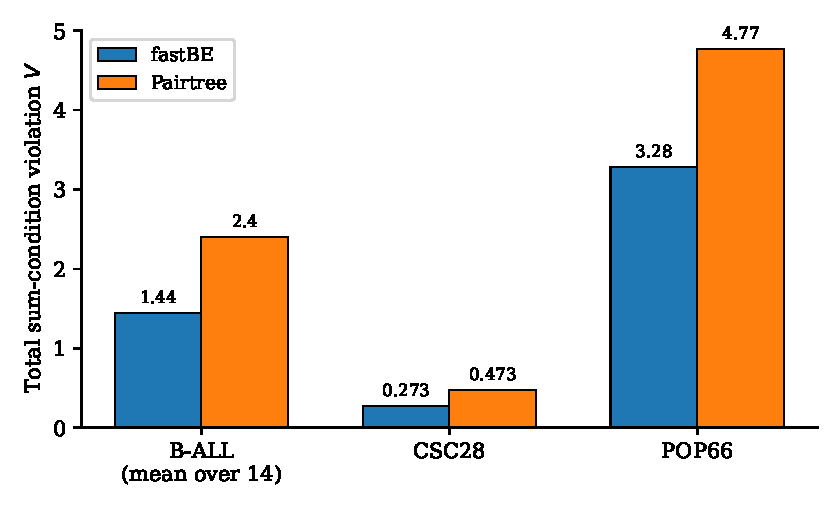
\includegraphics[width=0.75\textwidth]{figures/fig_sum_violation.pdf}
\caption{Total violation $V$ of the sum condition for phylogenies inferred by fastBE and Pairtree. On fourteen B-progenitor acute lymphoblastic leukaemia patients, fastBE reduces the mean total violation from 2.40 to 1.44. On the CSC28 colorectal xenograft the total violation drops from 0.473 to 0.273, and on the POP66 xenograft from 4.770 to 3.280.}
\label{fig:sum_violation}
\end{figure}
